\documentclass[a4paper,11pt]{article}

% Packages and settings {{{1
\usepackage[default,regular,semibold,scale=0.94]{sourceserifpro}
\usepackage[lining,scale=0.87]{FiraMono}
\usepackage[T1]{fontenc}
\usepackage[version=4]{mhchem}
\usepackage[font=small,labelfont=it,margin=15pt]{caption}
\usepackage{amsmath,bm,fullpage,parskip,graphicx,float,braket,setspace,subcaption}
\usepackage[dvipsnames]{xcolor}
\usepackage[style=chem-acs,subentry,doi]{biblatex}
\addbibresource{genesis.bib}
\graphicspath{{./figures/}}
\usepackage{xurl}   % must be after biblatex
\usepackage[exponent-product=\cdot]{siunitx}
\usepackage[symbol]{footmisc}
\usepackage{hyperref}
\hypersetup{
    colorlinks,
    linkcolor={red!50!black},
    citecolor={blue!60!black},
    urlcolor={blue!80!black}
}
\usepackage[capitalise,noabbrev]{cleveref}

\usepackage{usebib}
\newbibfield{entryset}
\bibinput{genesis}

\onehalfspacing
\DeclareSIUnit{\molar}{\textsc{m}}
\DeclareSIUnit{\ppm}{ppm}
% }}}1
% Newcommands {{{1 
\newcommand{\proton}{\ce{^{1}H}}
\newcommand{\carbon}{\ce{^{13}C}}
\newcommand{\nitrogen}{\ce{^{15}N}}
\newcommand{\CH}{\carbon{}--\proton{}}
\newcommand{\HC}{\proton{}--\carbon{}}
\newcommand{\NH}{\nitrogen{}--\proton{}}
\newcommand{\HN}{\proton{}--\nitrogen{}}
\newcommand{\HH}{\proton{}--\proton{}}
\newcommand{\todo}[1]{\textcolor{WildStrawberry}{#1}}
\newcommand{\autociteset}[1]{\autocite{\usebibentry{#1}{entryset}}}
\newcommand{\onejch}{{}^1\!J_{\ce{CH}}}
\newcommand{\njch}{{}^n\!J_{\ce{CH}}}
\newcommand{\onejnh}{{}^1\!J_{\ce{NH}}}
\newcommand{\theurl}{\url{https://nmr-genesis.co.uk}}
\newcommand*{\andro}{Spectra were obtained on a \SI{700}{\MHz} Bruker AV III equipped with a TCI H/C/N cryoprobe; the sample used was \SI{40}{\milli\molar} andrographolide in DMSO-$d_6$.}
\newcommand*{\grami}{Spectra were obtained on a \SI{700}{\MHz} Bruker AV III equipped with a TCI H/C/N cryoprobe; the sample used was \SI{40}{\milli\molar} gramicidin in DMSO-$d_6$.}
\newcommand*{\zolmi}{Spectra were obtained on a \SI{700}{\MHz} Bruker AV III equipped with a TCI H/C/N cryoprobe; the sample used was \SI{50}{\milli\molar} zolmitriptan in DMSO-$d_6$.}
% }}}1
% Counters for the combinatorics {{{1
\newcount\nmoda
\newcount\nmodb
\newcount\nmodc
\newcount\nmodd
\newcount\nmode
\newcount\nmoddup
\newcount\nmoddoublehom
\nmoda=2
\nmodb=3
\nmodc=5
\nmodd=9
\nmode=19
\nmoddoublehom=6
\nmoddup=\numexpr(\nmodc-1)
\newcommand{\ee}[1]{\the\numexpr#1\relax}
% }}}1

\begin{document}

\begin{center}   % Front matter
    \textbf{\Large Modular pulse programme generation for NOAH supersequences}

    \vspace{0.2cm}

    Jonathan R.\ J.\ Yong,\textsuperscript{1} {\=E}riks Kup{\v{c}}e,\textsuperscript{2} Tim D. W. Claridge\textsuperscript{1,*}

    \vspace{0.2cm}

    \textsuperscript{1} \textit{Chemistry Research Laboratory, Department of Chemistry, University of Oxford, Mansfield Road, Oxford, OX1 3TA, U.K.}

    \textsuperscript{2} \textit{Bruker UK Ltd., Banner Lane, Coventry, CV4 9GH, U.K.}

    \textsuperscript{*} \texttt{tim.claridge@chem.ox.ac.uk}

    \vspace{0.5cm} \hrule
\end{center}
\section*{Abstract}

\textit{(132 words)}

NOAH (NMR by Ordered Acquisition using \proton{}-detection) supersequences allow multiple 2D NMR datasets to be acquired in greatly reduced experiment durations through the elision of recovery delays.
In NOAH experiments, up to five ``modules'' can be combined, which means that there is a very large number of plausible supersequences (over 4000).
This renders the traditional method of pulse programme construction by hand wholly inadequate.
We introduce here a tool named GENESIS (GENEration of Supersequences In Silico), available via \theurl{}, which programmatically generates arbitrary NOAH supersequences compatible with Bruker spectrometers.
This not only allows users to obtain customised supersequences for specific applications, but also enables us to rapidly and effortlessly disseminate new NOAH modules (e.g.\ PSYCHE, 2D J) as well as improvements to old modules (e.g.\ \CH{} HMBC, \NH{} HMQC).

\section{Introduction}

Accelerating NMR data acquisition has in recent years proven a fruitful area for NMR pulse sequence and method development, particularly for $n$-dimensional ($n$D) NMR where raw data is acquired as a series of increments.
Developments in this area include (but are not limited to) ultrafast NMR\autociteset{ultrafast}, non-uniform sampling (NUS)\autociteset{nus}, multiple-FID experiments\autociteset{multifid}, and the shortening or elision of recovery delays\autociteset{reducedd1}.
In this paper, we focus on NOAH (NMR by Ordered Acquisition using \proton{}-detection) experiments,\autociteset{noah} which fall under the last two categories.
NOAH experiments consist of a series of up to five 2D experiments (``modules''), combined into one single ``supersequence'' which uses only one recovery delay for all modules.
This provides substantial (up to $4\times$) time savings compared to conventional acquisition, in which one recovery delay is used for each module (\cref{fig:noah_diagram}).

\begin{figure}
    \centering
    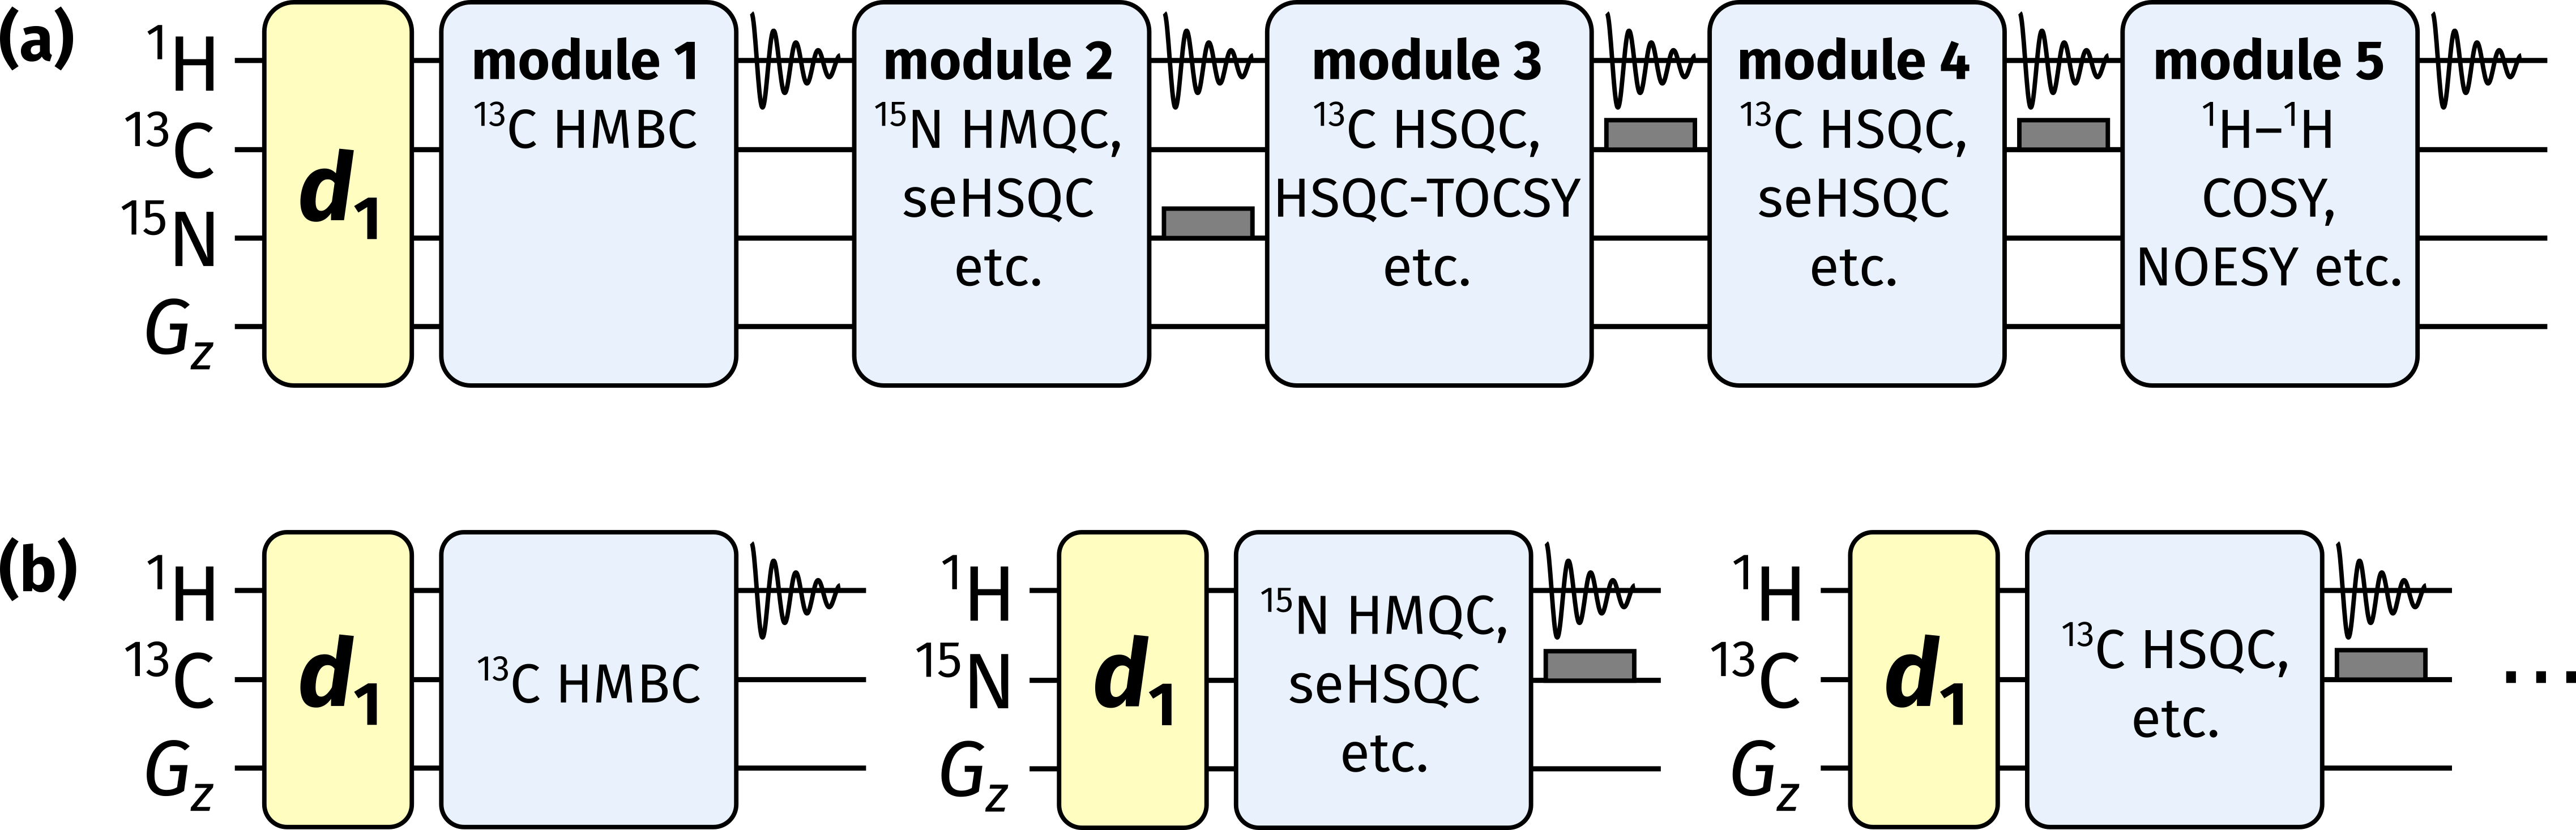
\includegraphics[width=0.8\textwidth]{noah_diagram.png}
    {\phantomsubcaption\label{fig:noah_diagram_noah}}
    {\phantomsubcaption\label{fig:noah_diagram_conventional}}
    \caption{
        \textbf{(\subref{fig:noah_diagram_noah})} Diagrammatic representation of a NOAH supersequence, where only one recovery delay ($d_1$) is used for the entire experiment.
        \textbf{(\subref{fig:noah_diagram_conventional})} Conventional 2D NMR data acquisition, where one recovery delay is used per dataset.
    }
    \label{fig:noah_diagram}
\end{figure}

Virtually all common 2D experiments have been implemented in NOAH supersequences to date, including HMBC, HSQC, HSQC-TOCSY, HMQC, COSY, TOCSY, NOESY, and ROESY.
Each module is given a one-letter code, such as `B' for HMBC, `S' for HSQC, `M' for HMQC, `C' for COSY, and so on.
The combinatorial nature of NOAH experiments means that there are a very large number of conceivable supersequences ranging from NOAH-2 to NOAH-5 (where the suffix indicates the number of modules).
In principle, this figure is on the order of $N^5$, where $N$ is the number of available modules: as of the time of writing, $N$N$\mathrm{e}$e\texttt{e} is 27, which in total yields more than 10 million NOAH supersequences.

For optimal data quality in terms of both sensitivity and artefact avoidance, there are certain conditions on NOAH supersequences.
Specifically, each NOAH module should ideally utilise only the specific magnetisation it requires: this allows it to be placed earlier in the supersequence.
As a concrete example, in the NOAH-2 SC supersequence (HSQC and COSY), the \HC{} HSQC module is designed to excite only the \proton{} nuclei directly attached to the 1.1\%-natural abundance \carbon{} and leave all other proton magnetisation (the ``bulk magnetisation'') along the equilibrium $+z$ axis.\autocite{SchulzeSunninghausen2014JACS}
A \HH{} COSY module (or TOCSY, or NOESY, etc.) can then draw on this bulk magnetisation, with almost no loss in sensitivity and without having to wait for the \carbon{}-bound protons to relax.
Conversely, if the COSY module were placed first, the \carbon{}-bound proton magnetisation would not survive for use in the HSQC: thus, the HSQC module in a NOAH-2 CS would display severe sensitivity losses, as compared to in a NOAH-2 SC.
More subtle factors are also abound, such as in the SBC sequence\autocite{Kupce2017ACIE}, where COSY intensities are modulated by $T_2$ relaxation and $J_{\ce{HH}}$ evolution.
The alternative BSC arrangement\autocite{Kupce2018CC}, especially with isotropic ``ASAP'' mixing applied before the COSY, circumvents this issue and has become the preferred implementation for HMBC/HSQC combinations\autocite{Claridge2019MRC}.

Considerations such as these restrict the set of ``effective'' NOAH supersequences.
Even so, the original NOAH paper alone suggests a figure of 285\autocite{Kupce2017ACIE}, and the number of available modules has only grown since then.
By our calculations, as of the time of writing, there are
\(\ee{(\nmoda*\nmodb*\nmodc*\nmodd*\nmode)-1-(\nmoda+\nmodb+\nmodc+\nmodd+\nmode-5)-((\nmoda-1)*(\nmodb-1)*(\nmodc-1)*(\nmodd-1)*\nmoddoublehom)-(\nmode-1)-(\nmoda*\nmodb*\nmoddup*\nmode)+(\nmoddup)}\)
``optimal'' NOAH supersequences (\cref{sec:combinations}).
Constructing every one of these supersequences ``by hand'' is clearly unreasonable.
Consequently, it has not been possible to disseminate an exhaustive series of pulse programmes: we have so far had to limit ourselves to a handful of ``typical'' supersequences, which may or may not be applicable to users' needs.
To solve this problem, we sought to \textit{programmatically} generate NOAH pulse programmes, in a way which makes new combinations as easy as possible to set up and minimises the chances of human error.
We term this approach GENESIS (GENEration of Supersequences In Silico).
The implementation of this is a single web page (\cref{fig:screenshot}), accessible via \theurl{}, which can construct virtually any supersequence one might want.
The regular user interface is designed to only produce ``optimal'' supersequences: thus, for example, it is not possible to create the CS or SBC supersequences discussed earlier.
This is most useful for ordinary users who wish to follow established best practices.
For more advanced usage, enabling ``developer mode'' will remove these limitations, allowing any arbitrary combination of modules to be created.

\begin{figure}
    \centering
    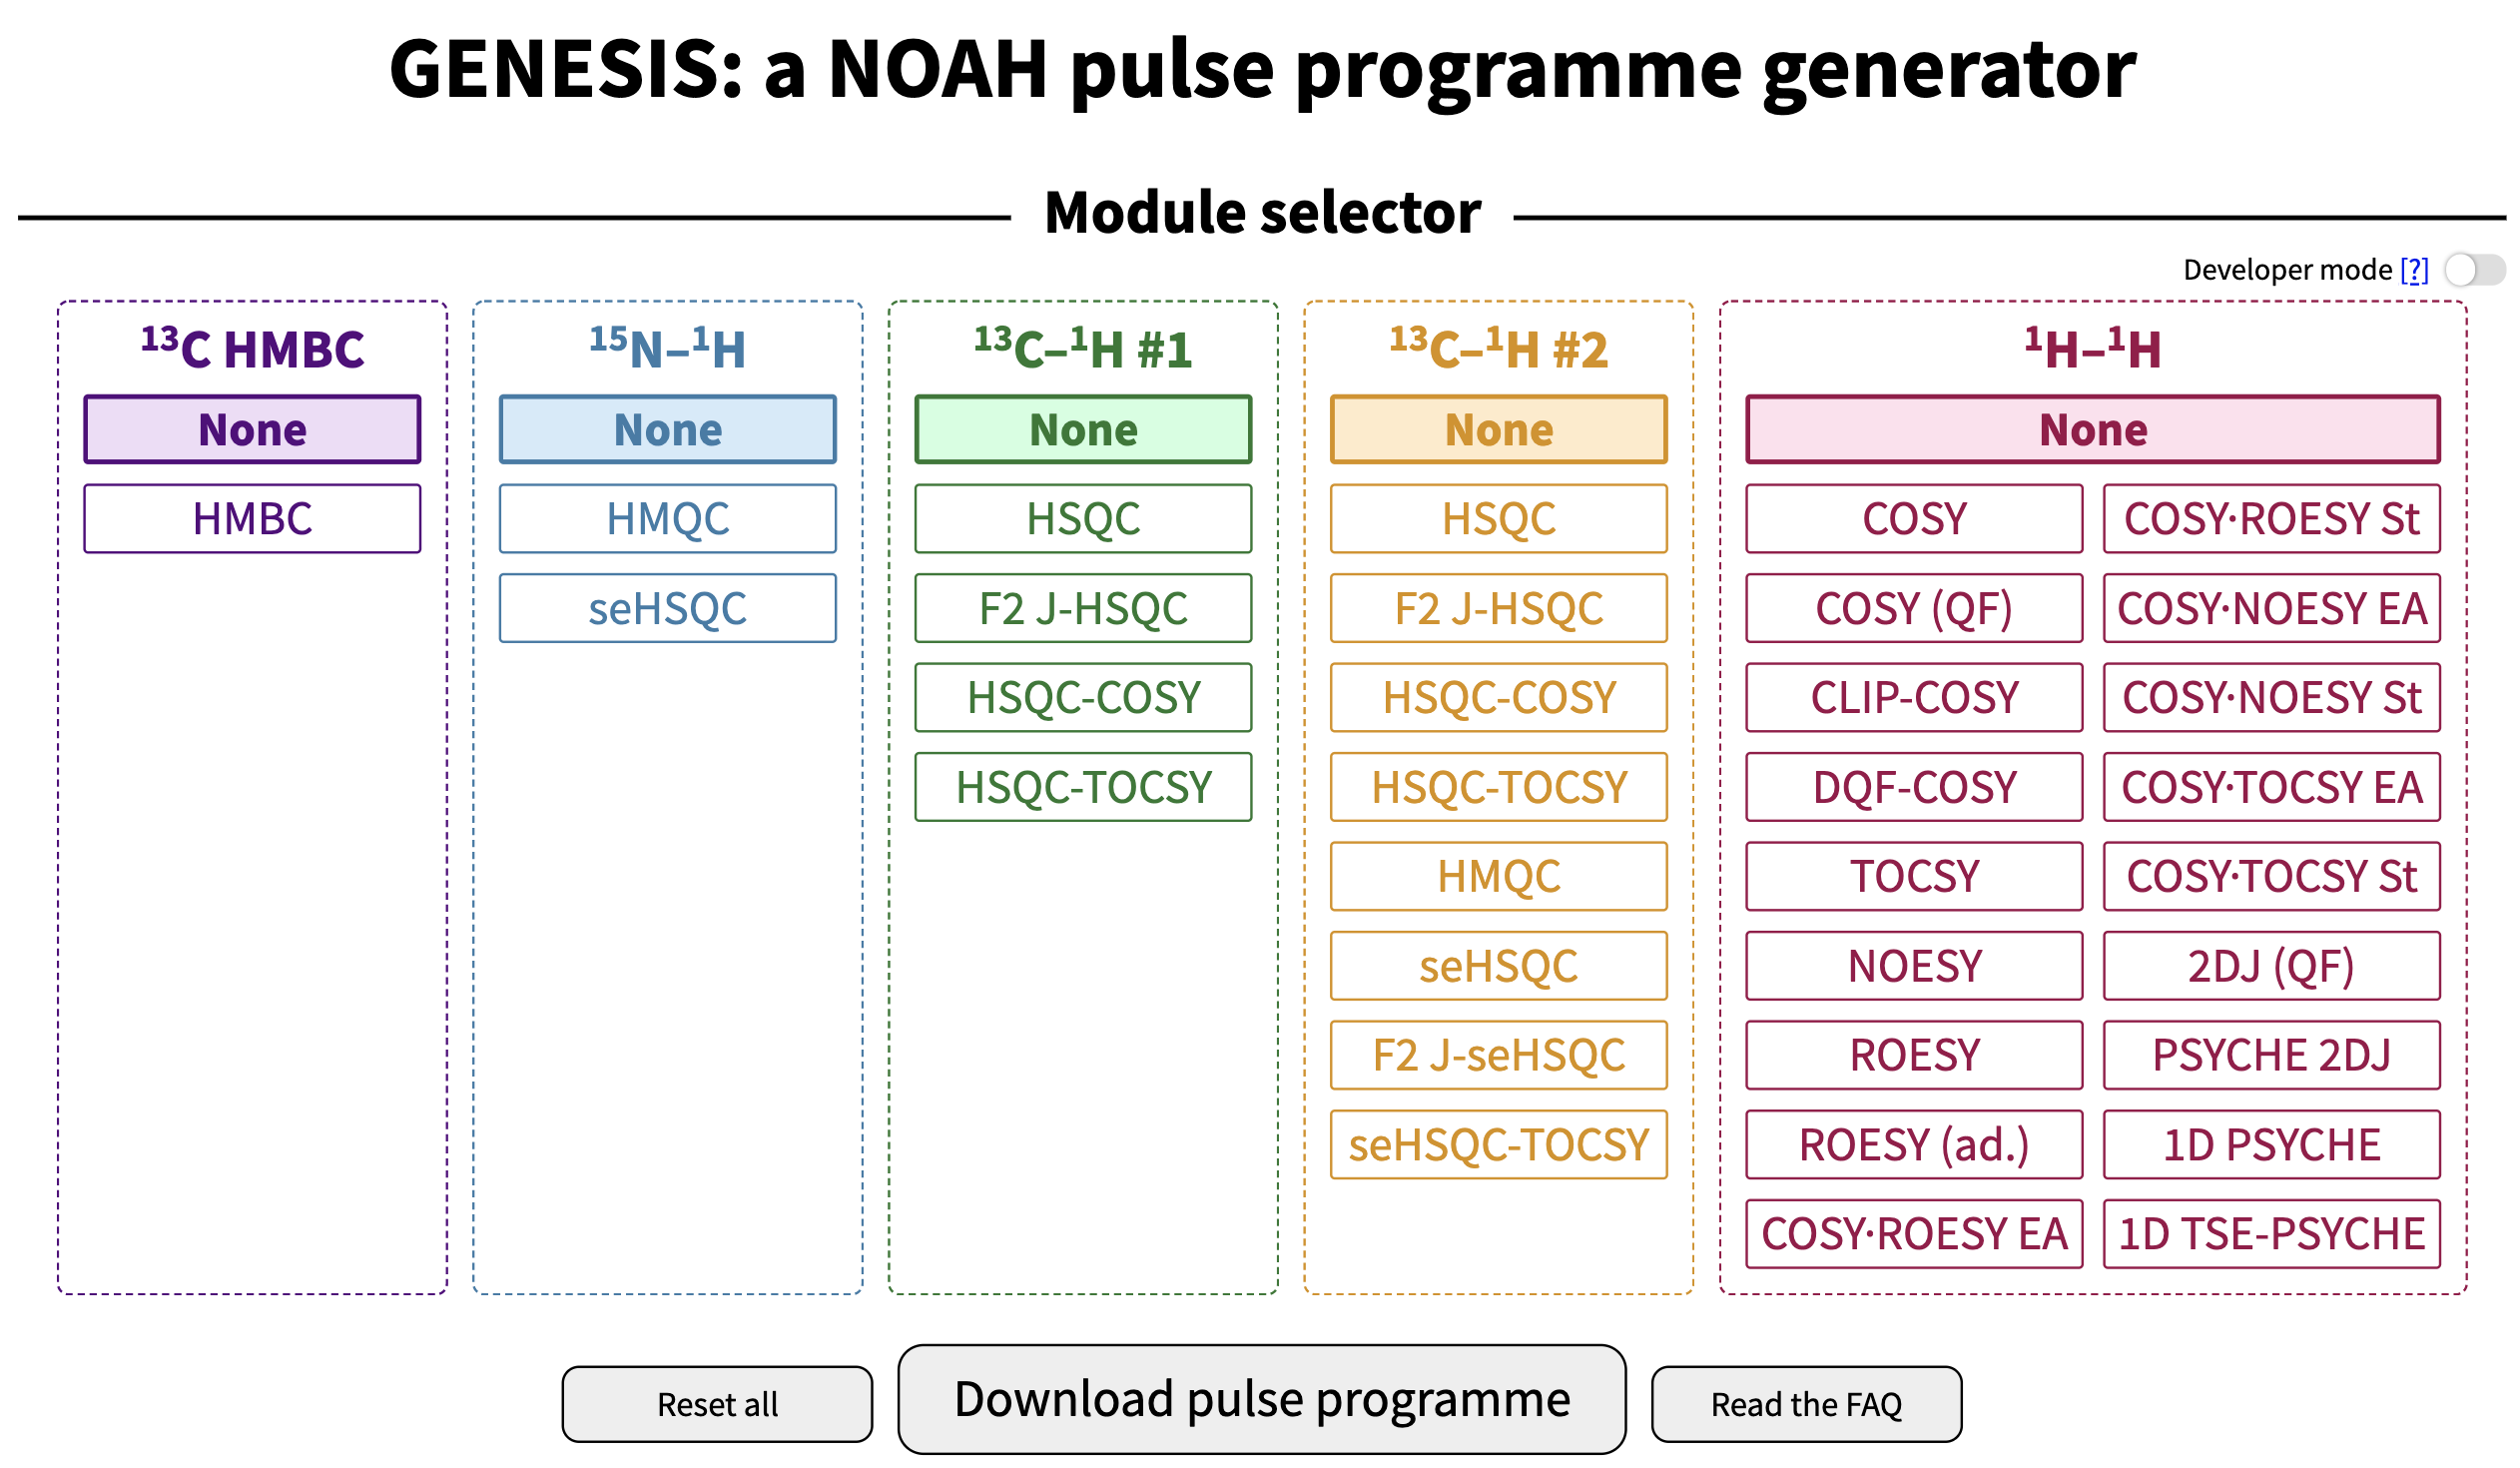
\includegraphics[width=0.8\textwidth]{screenshot.png}
    \caption{
        A screenshot of the GENESIS web interface.
        Visible here are the module choices, the ``developer mode'' toggle, and buttons for downloading the pulse programme.
    }
    \label{fig:screenshot}
\end{figure}

\section{Implementation details}

We begin with a brief discussion of how the GENESIS approach works.
The pulse programme generation code itself is written in TypeScript (version 4.2.3, Microsoft), which is compiled to JavaScript (formally ECMAScript 2015, or ``ES6'') and then executed directly in a client's browser; there is no server-side code.
The web browser shows a list of modules for users to choose from, using accessible and familiar names such as HMBC, HSQC, and so on (\cref{fig:screenshot}).
Internally, these are mapped to a series of \texttt{NOAHModule} objects, each of which contain module-specific information, such as its abbreviation (usually one letter, but some are longer e.g. $\mathrm{S^T}$/\texttt{St} for HSQC-TOCSY), parameter definitions, the pulse programme for the module itself, and the appropriate AU programme to be used for processing. 

\begin{figure}
    \centering
    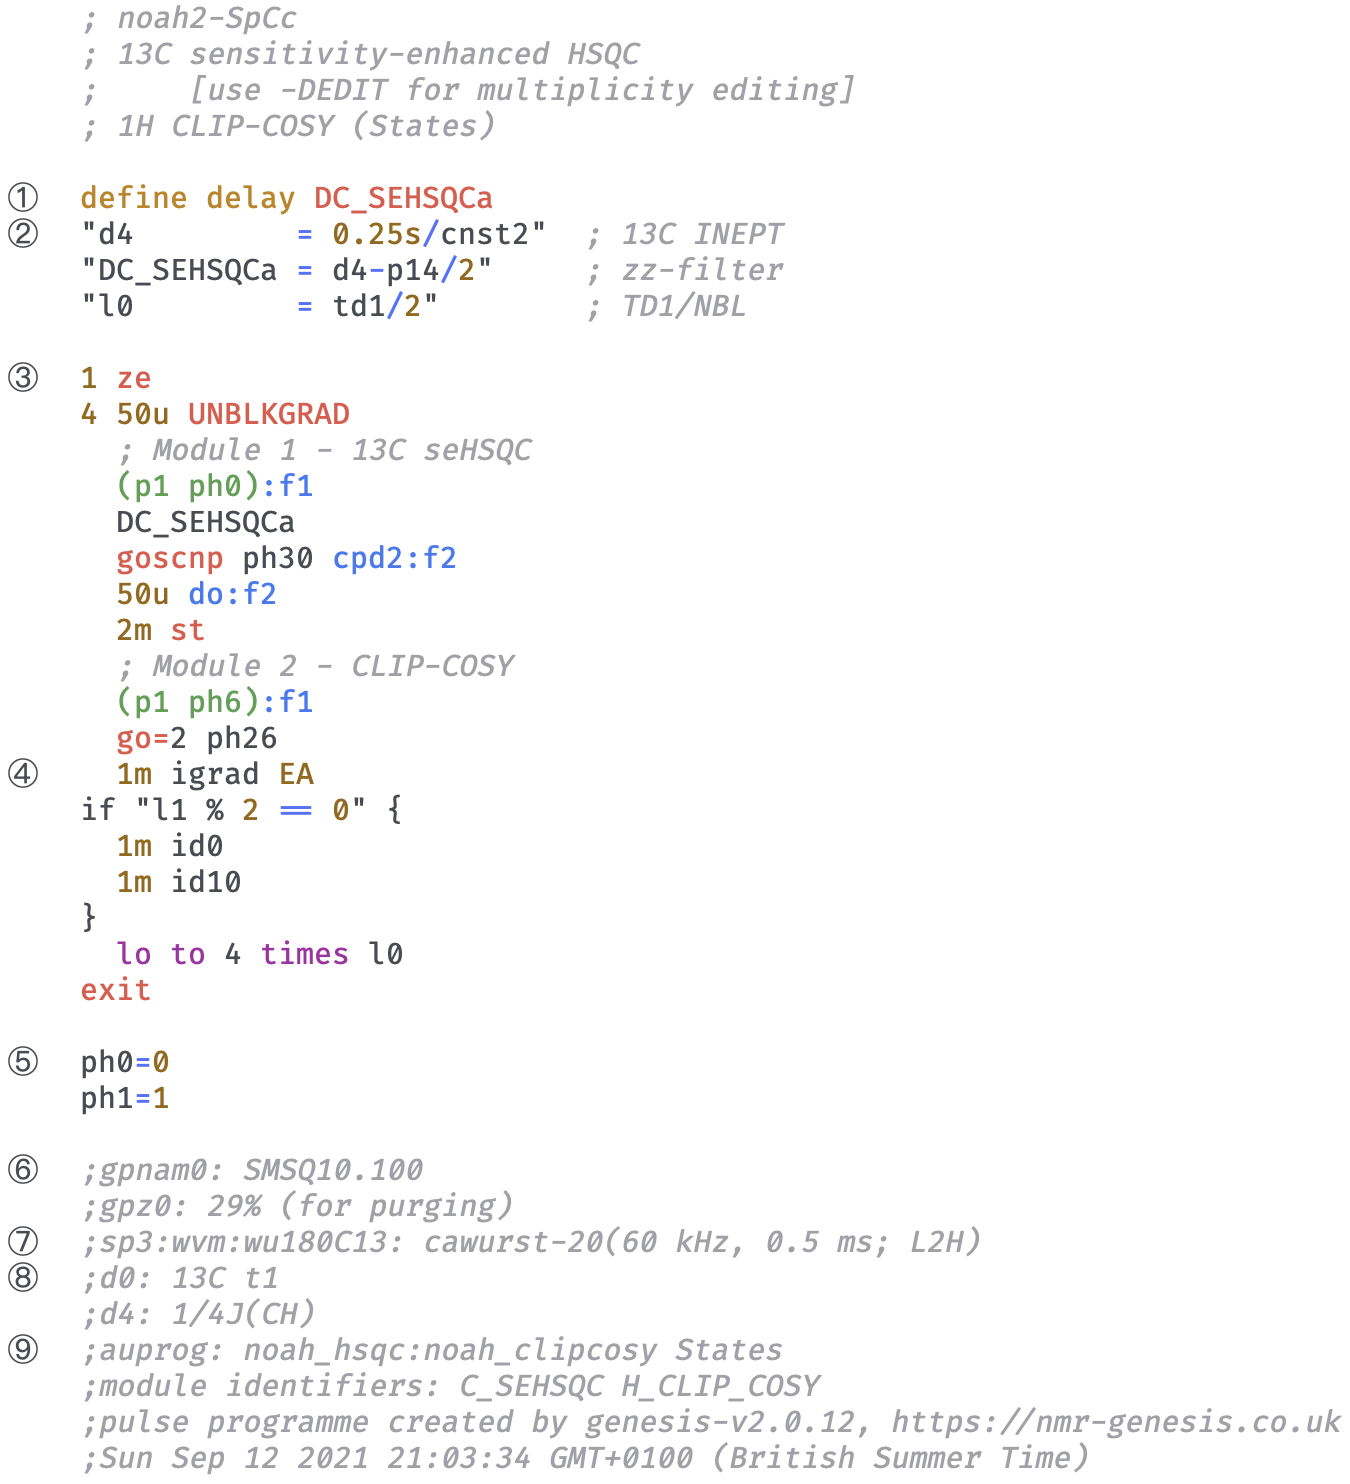
\includegraphics[width=0.8\textwidth]{pulprog_code.png}
    \caption{
        Abridged pulse programme for a NOAH-2 $\mathrm{S^+C^c}$ supersequence (\carbon{} seHSQC + CLIP-COSY).
        Specific sections of interest are numbered on the left.
        \textbf{(1)} Module-specific delays are given unique identifiers to prevent clashes and to improve readability.
        \textbf{(2)} TopSpin parameters (delays such as \texttt{d4}) are standardised between modules.
        \textbf{(3)} The pulse programme instructions themselves begin here.
        \textbf{(4)} $t_1$ incrementation and echo--antiecho gradient inversion is carried out with the appropriate frequency (once per loop or once per two loops).
        \textbf{(5)} Pulse and receiver phase cycles are standardised between modules.
        \textbf{(6)} Comments for gradient pulses are compatible with the TopSpin \texttt{gppp} script.
        \textbf{(7)} Instructions for generating shaped pulses using TopSpin's WaveMaker software.
        \textbf{(8)} Comments describing each parameter appear in the parameter setup screen.
        \textbf{(9)} Instructions for processing AU programmes (\cref{subsec:splitx_au}) are encoded here, along with information about the specific modules used and a timestamp which ensures reproducibility.
    }
    \label{fig:pulprog_code}
\end{figure}

Using this information, GENESIS then constructs the pulse programme in several steps (\cref{fig:pulprog_code}):

\begin{itemize}
    \item Header comments including information about the pulse programme and constituent modules;
    \item The preambles, which contains header comments including information about the pulse programme and constituent modules, as well as parameter definitions, are first collated.
        Particular care is taken to avoid duplicating parameter definitions which are used in multiple modules.
    \item The main section, which contains the actual instructions corresponding to the pulse sequence, is then put together.
        This is done mostly by simply concatenating individual modules together, although there are also context-sensitive blocks placed \textit{between} modules such as ASAP mixing\autocite{Claridge2019MRC} in BSX-type supersequences, or purge pulses and gradients.
    \item Appropriate looping and incrementation of parameters such as phase cycles, $t_1$ delays, and gradient pulses for echo--antiecho selection is added at the end of the main section.
    \item Additional comments containing descriptive text for parameters (displayed in TopSpin's \texttt{ased} parameter setup screen), as well as gradient and shaped pulse information (which allow direct setup using the \texttt{gppp} and \texttt{wvm} commands), are added at this stage.
        These are collated by scanning the main section for TopSpin parameters (e.g.\ delays, pulses, gradients) and obtaining their descriptions from a lookup table.
    \item Finally, to ensure full reproducibility in the pulse programme generation, we also specify the exact modules used in the pulse programme, the GENESIS version number, and a timestamp.
\end{itemize}

The website further contains a series of frequently asked questions and instructions on how to set NOAH experiments up.
It also offers download links for the AU scripts used for processing, as well as the new Python script used for toggling non-uniform sampling on/off (\texttt{noah\_nus2.py}).

\subsection{Standardisation of parameter meanings}

An immediate problem of directly concatenating pulse programme texts from different modules is that a given parameter in one module may take on a different value in another module.
As a necessary step to prevent such clashes, we have fully standardised all parameters used in the GENESIS pulse programmes.
These include pulse widths (\texttt{p}), delays (\texttt{d}), constants (\texttt{cnst}), $z$-gradient amplitudes (\texttt{gpz}), and phase cycles (\texttt{ph}).
Thus, \texttt{d2} is always $1 / (2 \cdot \onejch)$, and \texttt{d4} is always $1 / (4 \cdot \onejch)$.
Where possible, we have chosen meanings that are similar to those in the standard library of Bruker pulse programmes.
However, there are invariably some small deviations: for example, the $\Delta'$ delay in the \carbon{} sensitivity-enhanced HSQC (which can range from $1/(8 \cdot\onejch)$ to $1/(4 \cdot\onejch)$) is \texttt{d24} in the standard library, but we have chosen \texttt{d6} because \texttt{d24} is reserved for $1 / (4 \cdot \onejnh)$.

In place of module-specific delays which are often called \texttt{DELTA1}, \ldots{} in standard library sequences, we have chosen to define new identifiers with more human-readable names inside the pulse programme itself.
Thus, the delays in a HSQC sequence might be called \texttt{DC\_HSQC1}, \ldots{}, where the first \texttt{C} indicates the indirect-dimension nucleus (\carbon{}).

While this was primarily implemented in order to facilitate pulse programme construction, this standardisation also makes it far easier for users to set up a series of different supersequences, as virtually every parameter value can simply be reused.
In principle, it is possible to set up a single ``prototype'' parameter set which already has every parameter set up; to run a different NOAH experiment, one need only change \texttt{PULPROG}, \texttt{TD1}, and \texttt{NBL}.

\subsection{Choice of module `versions'}

Another potential issue is that different versions of a pulse sequence often exist.
A simple example is the $zz$-HMBC\autocite{Kupce2018CC,Kupce2019JMR}, where the $zz$-filter element is used to retain \carbon{}-bound and optionally \nitrogen{}-bound \proton{} magnetisation, depending on what modules follow.
Since the user only specifies that they want a HMBC module and not the exact details of the $zz$-filter, the GENESIS code must in effect make this choice for the user.
The sensitivity-enhanced HSQC (seHSQC, abbreviated `$\mathrm{S^+}$'/\texttt{Sp}) presents a more nuanced case.
If the seHSQC module is followed by one or more homonuclear modules such as a COSY or NOESY, then the ZIP-seHSQC\autocite{Hansen2021AC,Yong2021JMR} should be used, as this preserves the requisite magnetisation for the later modules.
However, if the seHSQC module is used last in the sequence, then the original Cavanagh--Rance--Kay seHSQC\autociteset{sehsqc} should be used in order to maximise sensitivity.
If necessary, this ``intelligent'' module selection can be circumvented by entering ``developer mode'', where the user is free to pick exactly which version of a module they want to include.
\todo{(Figure X depicts the decision process for the HMBC and seHSQC modules...)}


\section{Other NOAH improvements}

A substantial benefit of the GENESIS approach is that it provides a single source for all NOAH pulse sequences and processing scripts, which are always in sync with one another.
This allows us to rapidly disseminate new NOAH developments to users, independently from TopSpin's own release cycle, and without needing to write an entire paper about them.
The initial GENESIS release already contains a number of such improvements, some of which we detail below.

\subsection{Suppression of one-bond artefacts in HMBC}

\begin{figure}[ht]
    \centering
    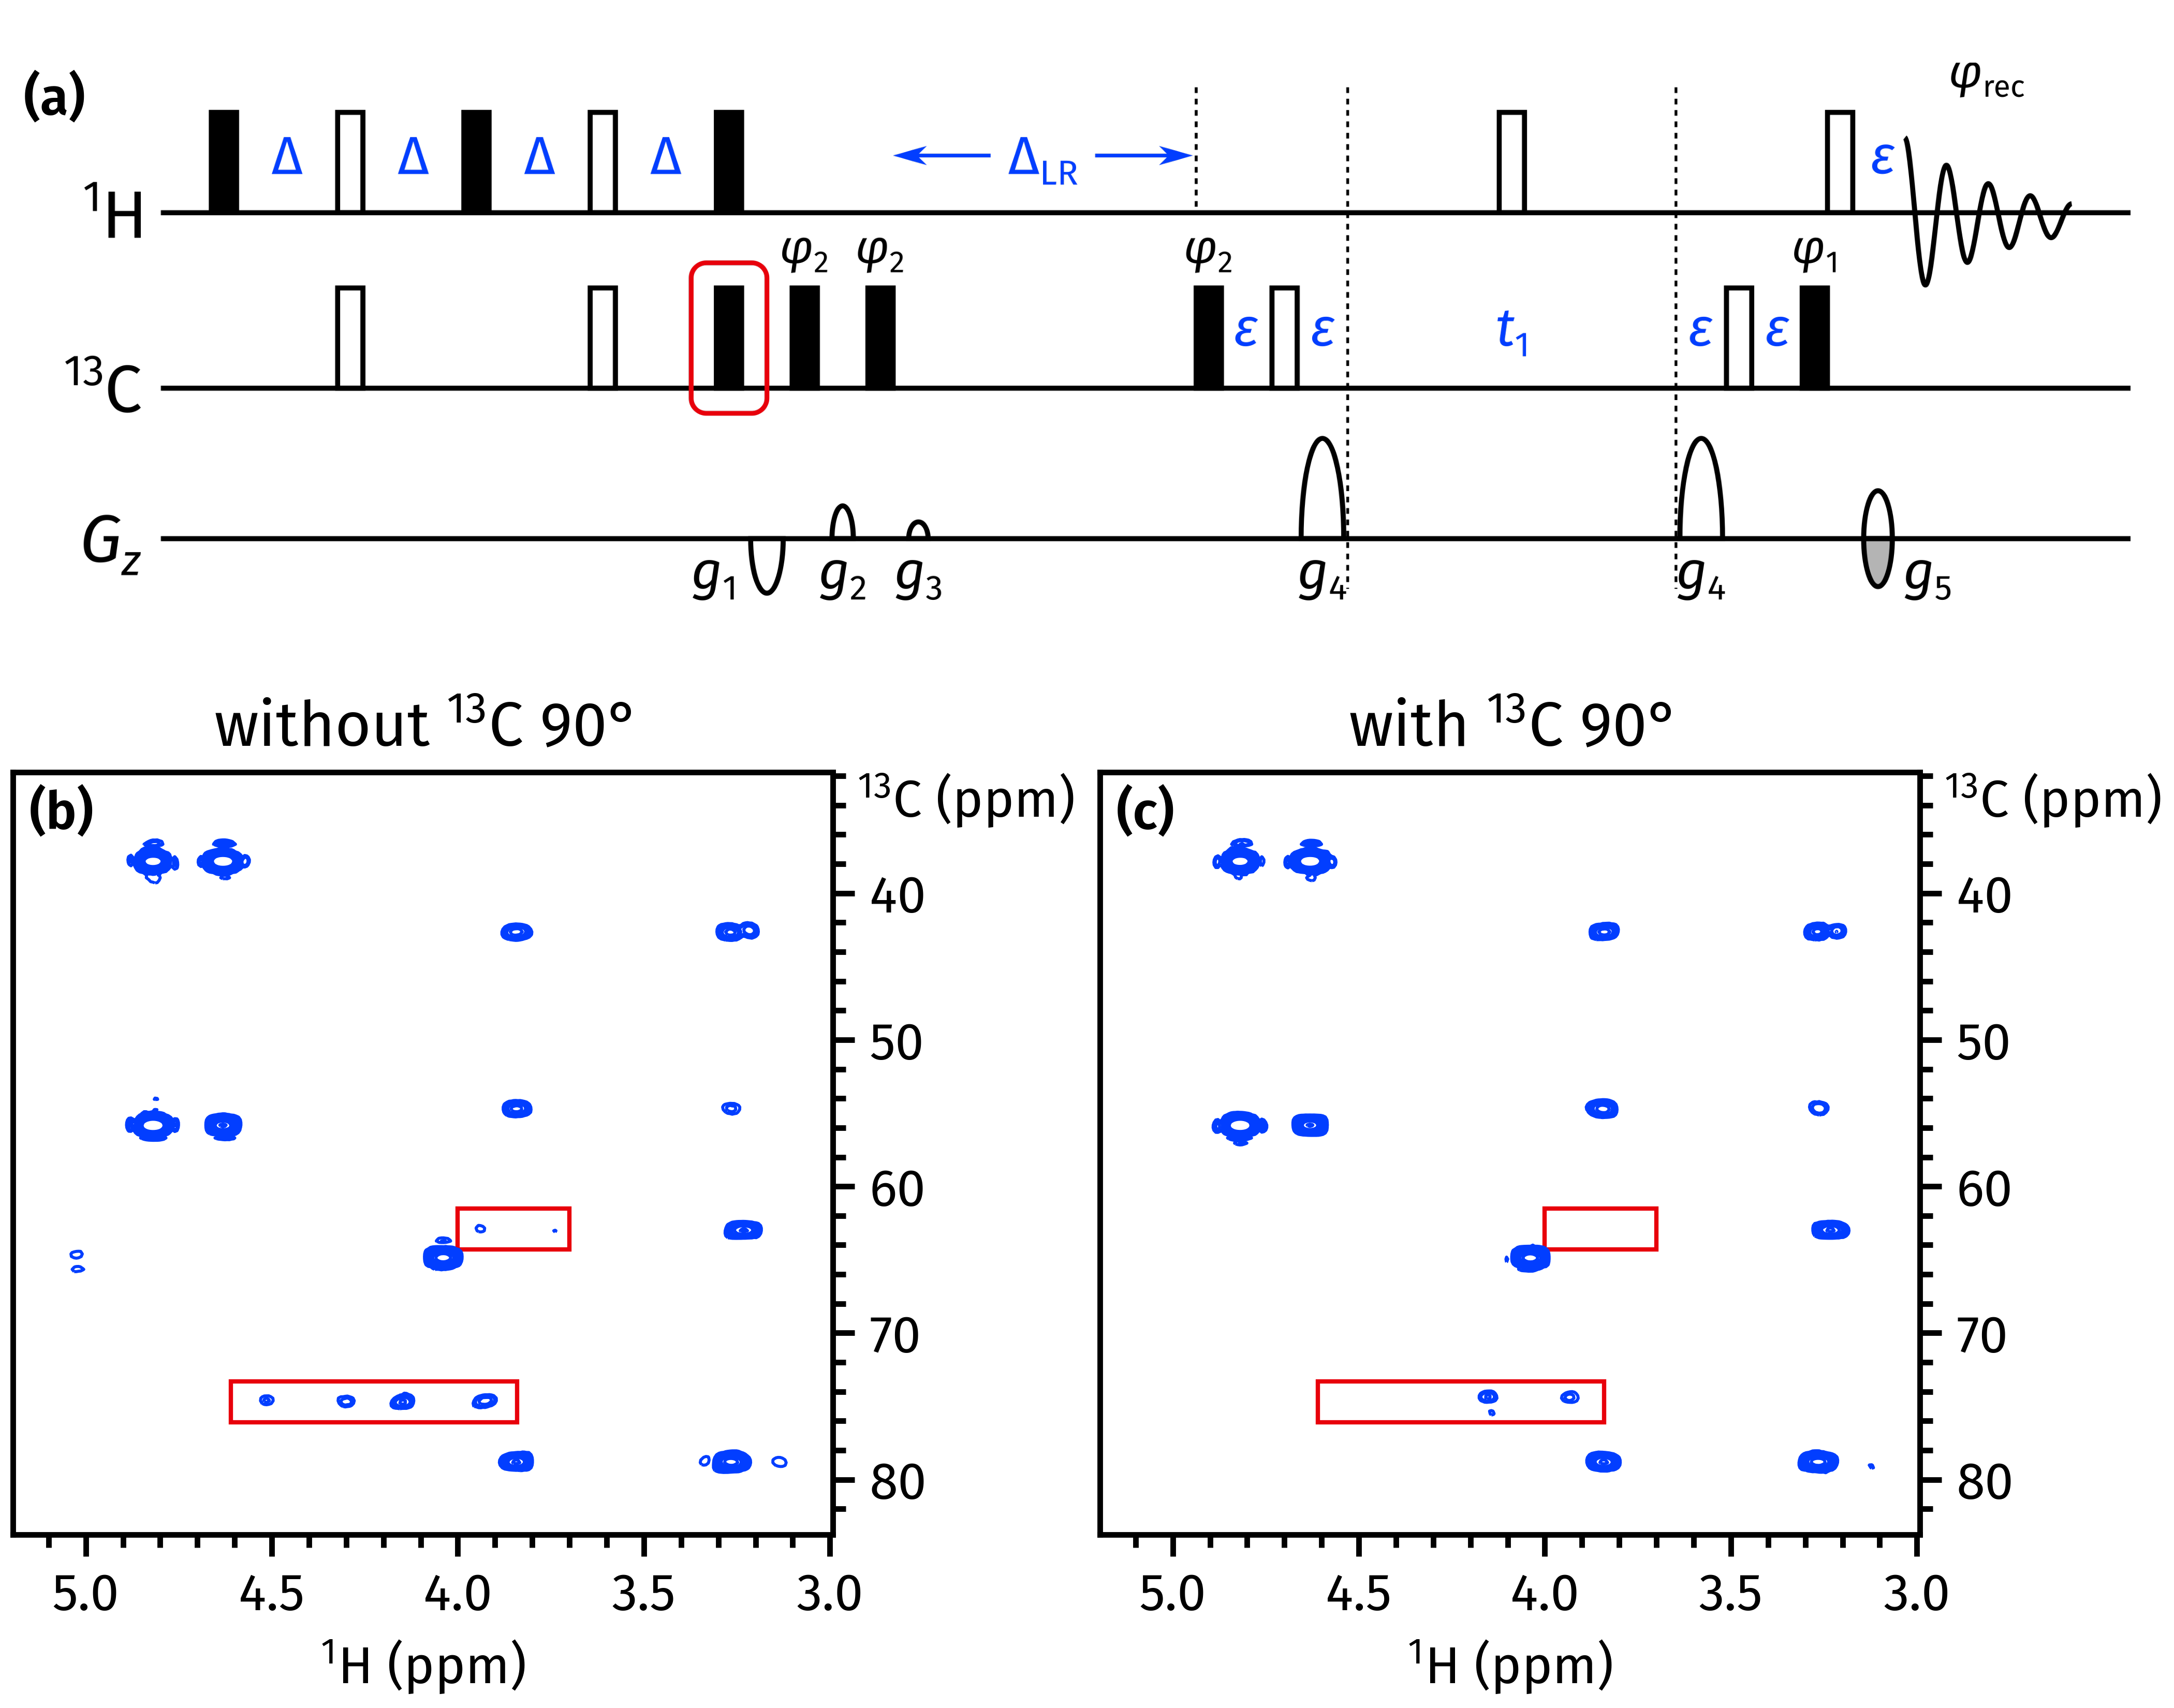
\includegraphics[width=0.7\textwidth]{hmbc_comp.png}
    {\phantomsubcaption\label{fig:hmbc_comp_pulprog}}
    {\phantomsubcaption\label{fig:hmbc_comp_before}}
    {\phantomsubcaption\label{fig:hmbc_comp_after}}
    \caption{
        \textbf{(\subref{fig:hmbc_comp_pulprog})} The NOAH $zz$-HMBC pulse sequence, with the newly added \carbon{} \ang{90} pulse highlighted in red.
        The delays are $\Delta = 1/(4 \cdot \onejch)$ and $\Delta_{\text{LR}} = 1/(2 \cdot \njch)$; $\varepsilon$ is the minimum time required for a gradient plus the subsequent recovery delay.
        Phase cycling is performed as follows: $\phi_1 = x, -x$; $\phi_2 = x, x, -x, -x$; $\phi_{\text{rec}} = x, -x, -x, x$.
        All gradients have duration \SI{1}{ms}; amplitudes as a fraction of the maximum gradient strength (\SI{55.7}{G\per\cm}) are as follows: $g_1 = -15\%$; $g_2 = 10\%$; $g_3 = 5\%$; $g_4 = 80\%$; $g_5 = \pm 40.2\%$.
        \textbf{(\subref{fig:hmbc_comp_before})} HMBC spectrum obtained using the original $zz$-HMBC module, i.e.\ without the added \ang{90} pulse.
        $\onejch{}$ artefacts are highlighted in red boxes.
        \textbf{(\subref{fig:hmbc_comp_after})} HMBC spectrum obtained with the added \ang{90} pulse.
        \andro{}
    }
    \label{fig:hmbc_comp}
\end{figure}

The $zz$-HMBC module is ordinarily placed first in a supersequence, where the $zz$-filter element serves to preserve magnetisation of protons directly coupled to \carbon{} and/or \nitrogen{}.\autocite{Kupce2018CC,Kupce2019JMR}
Specifically, the $zz$-filter acts as a \ang{90} excitation pulse on uncoupled protons, while leaving coupled protons along $+z$.
This is largely accomplished in practice, as evidenced by the fact that the intensities in subsequent HSQC-type modules are barely perturbed.
However, not all of the coupled magnetisation is perfectly retained: in particular, the $zz$-filter also generates a degree of \textit{antiphase} magnetisation of the form $2\mathrm{H}_x\mathrm{C}_z$.
This antiphase magnetisation is later refocused during the low-pass J-filter (LPJF) to give in-phase magnetisation, eventually ending up as one-bond correlation artefacts in the HMBC spectrum (\cref{fig:hmbc_comp_before}).

A simple solution to this is to add a \carbon{} \ang{90} pulse at the end of the $zz$-filter (\cref{fig:hmbc_comp_pulprog}): this converts any antiphase magnetisation to double- or zero-quantum magnetisation, which is later destroyed by the LPJF.
This idea has previously been used by Luy and coworkers in CLIP-HSQC experiments to remove antiphase contributions prior to FID detection.\autocite{Enthart2008JMR}
In the event, this small modification proved to have a large impact, almost completely suppressing the $\onejch$ artefacts (\cref{fig:hmbc_comp_after}).
\todo{Further comparisons of artefact intensity are provided in the SI.}

\subsection{\texorpdfstring{\nitrogen{}}{15N} HMQC gradient scheme}

\begin{figure}[ht]
    \centering
    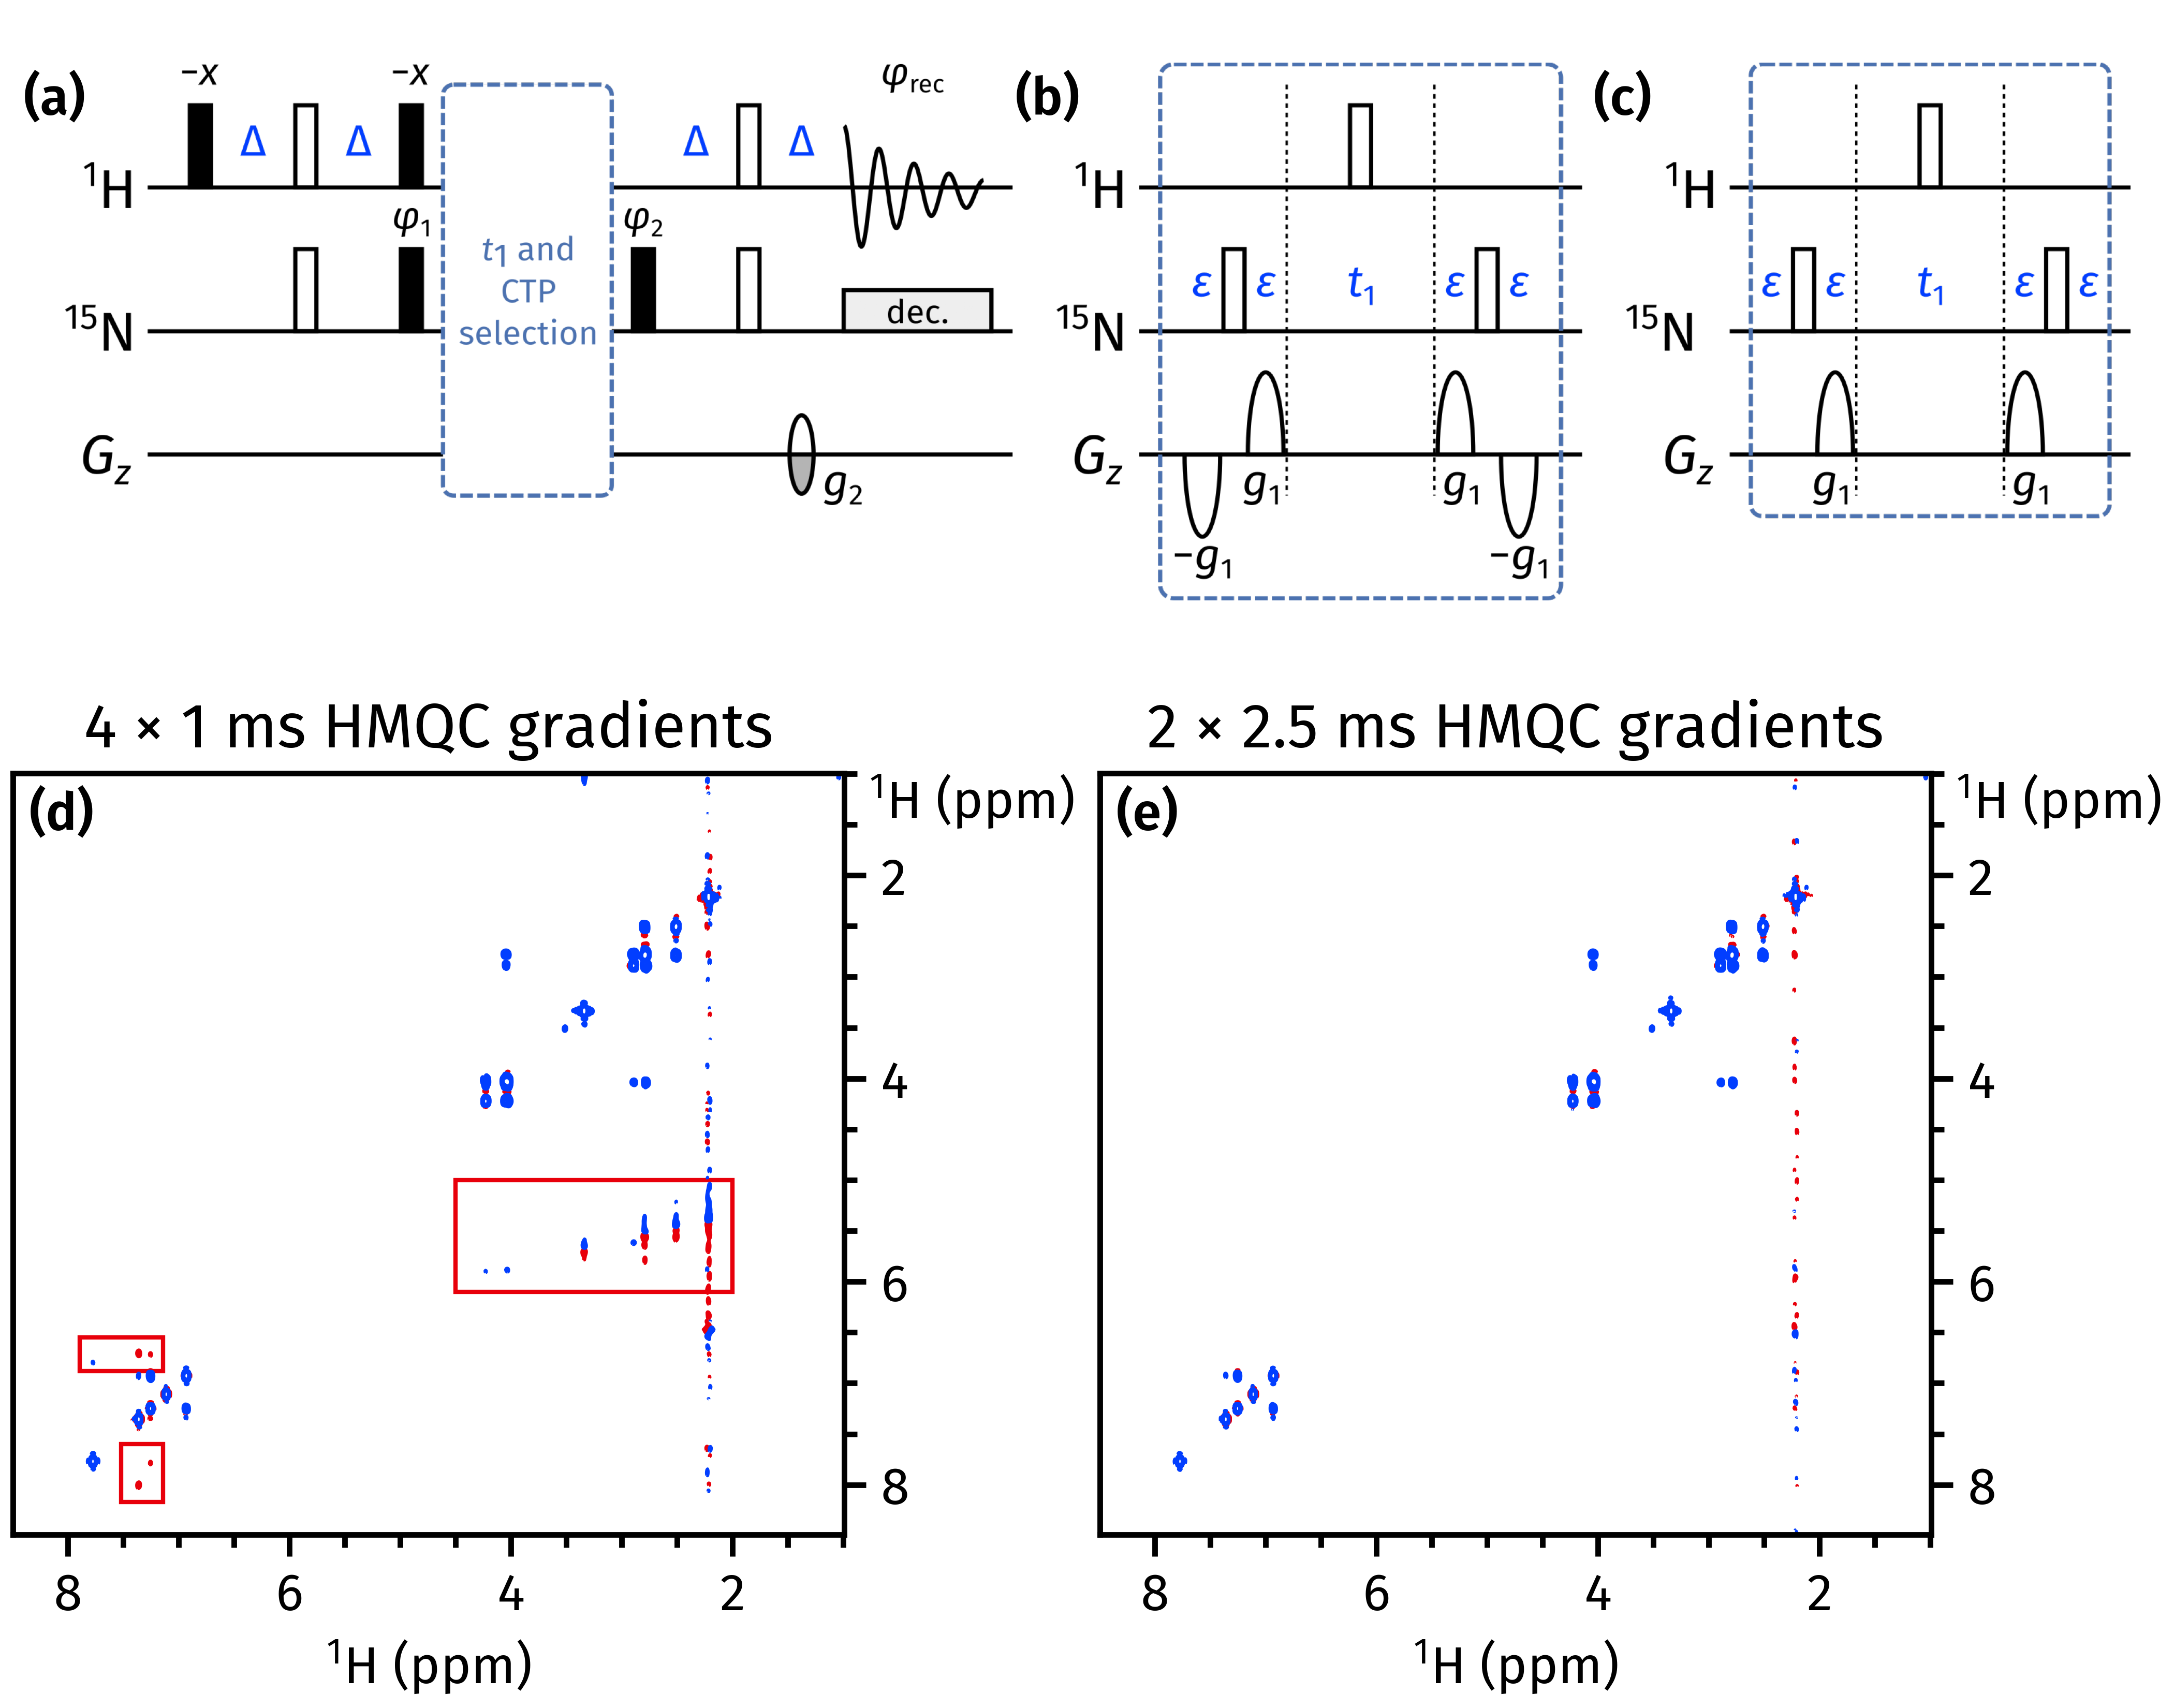
\includegraphics[width=0.7\textwidth]{hmqc_comp.png}
    {\phantomsubcaption\label{fig:hmqc_comp_pulprog}}
    {\phantomsubcaption\label{fig:hmqc_comp_pulprog_before}}
    {\phantomsubcaption\label{fig:hmqc_comp_pulprog_after}}
    {\phantomsubcaption\label{fig:hmqc_comp_spec_before}}
    {\phantomsubcaption\label{fig:hmqc_comp_spec_after}}
    \caption{
        \textbf{(\subref{fig:hmqc_comp_pulprog})} A general outline of the NOAH \nitrogen{} HMQC module.
        $g_2$ has a duration which matches that of $g_1$ (explained below), and an amplitude of $\pm n \cdot 8.1\%$, where $n$ is the number of CTP gradients bracketing the $t_1$ period.
        $g_1$ has an amplitude of $80\%$ in all cases.
        All other symbols have the same meaning as in \cref{fig:hmbc_comp}.
        \textbf{(\subref{fig:hmqc_comp_pulprog_before})} The previously published coherence selection scheme for the HMQC module, with four gradients each of duration \SI{1}{ms}.
        \textbf{(\subref{fig:hmqc_comp_pulprog_after})} The new coherence selection scheme for the HMQC module, with two gradients each of duration \SI{2.5}{ms}.
        \textbf{(\subref{fig:hmqc_comp_spec_before})--(\subref{fig:hmqc_comp_spec_after})} CLIP-COSY spectra obtained from a NOAH-3 $\mathrm{MS^+C^c}$ supersequence (\nitrogen{} HMQC + \carbon{} seHSQC + CLIP-COSY), acquired with the gradient schemes shown in (\subref{fig:hmqc_comp_pulprog_before}) and (\subref{fig:hmqc_comp_pulprog_after}) respectively.
        The wing artefacts in the former spectrum are highlighted in red boxes.
        \zolmi{}
    }
    \label{fig:hmqc_comp}
\end{figure}

We have recently described the occurrence of ``wing artefacts'' in homonuclear modules, which arise from bulk magnetisation which evolves during either half of $t_1$ in a preceding heteronuclear module.\autocite{Yong2021JMR}
These artefacts can be removed in an elegant manner by ensuring that each half of $t_1$ in a HMQC/HSQC/seHSQC module contains coherence transfer pathway (CTP) gradients of equal sign and magnitude, which makes sure that any bulk magnetisation undergoing net evolution during $t_1$ is dephased.

At the same time, it is also important that the final gradient in the heteronuclear module have as large an amplitude as possible, since this gradient is responsible for dephasing bulk magnetisation that is not returned to $+z$ just prior to the detection period.
In order to accomplish this, the previous \nitrogen{} HMQC module used bipolar opposing gradients in either half of $t_1$, a scheme which allows the final refocusing CTP gradient $g_2$ to have an amplitude of $4\gamma_{\ce{N}} / \gamma_{\ce{H}}$ (\cref{fig:hmqc_comp_pulprog,fig:hmqc_comp_pulprog_before}).
Although this leads to excellent artefact suppresion in the \nitrogen{} HMQC itself, wing artefacts are apparent in downstream modules (\cref{fig:hmqc_comp_spec_before}), because the opposing gradients cancel each other out and do not enforce any CTP selection on the bulk magnetisation.

The solution to this is to only use two gradients during $t_1$ (one in either half), but to \textit{lengthen} their duration such that the final gradient $g_2$ provides sufficient dephasing in the HMQC itself (\cref{fig:hmqc_comp_pulprog_after}).
This strategy was previously described for the \nitrogen{} seHSQC;\autocite{Yong2021JMR} here we have also applied it to the HMQC with success (\cref{fig:hmqc_comp_spec_after}).

\subsection{PSYCHE and 2DJ modules}

In previous work,\autocite{Yong2021JMR} we described how the sensitivity of some \nitrogen{} modules, particularly the HMQC, could be improved through the use of $k$-scaling.\autocite{PerezTrujillo2007MRC}
This entails a reduction in the number of $t_1$ increments (by a factor of $k$), in return for a corresponding increase in the number of transients per increment, with no overall change in the experimental time.

\begin{figure}[ht]
    \centering
    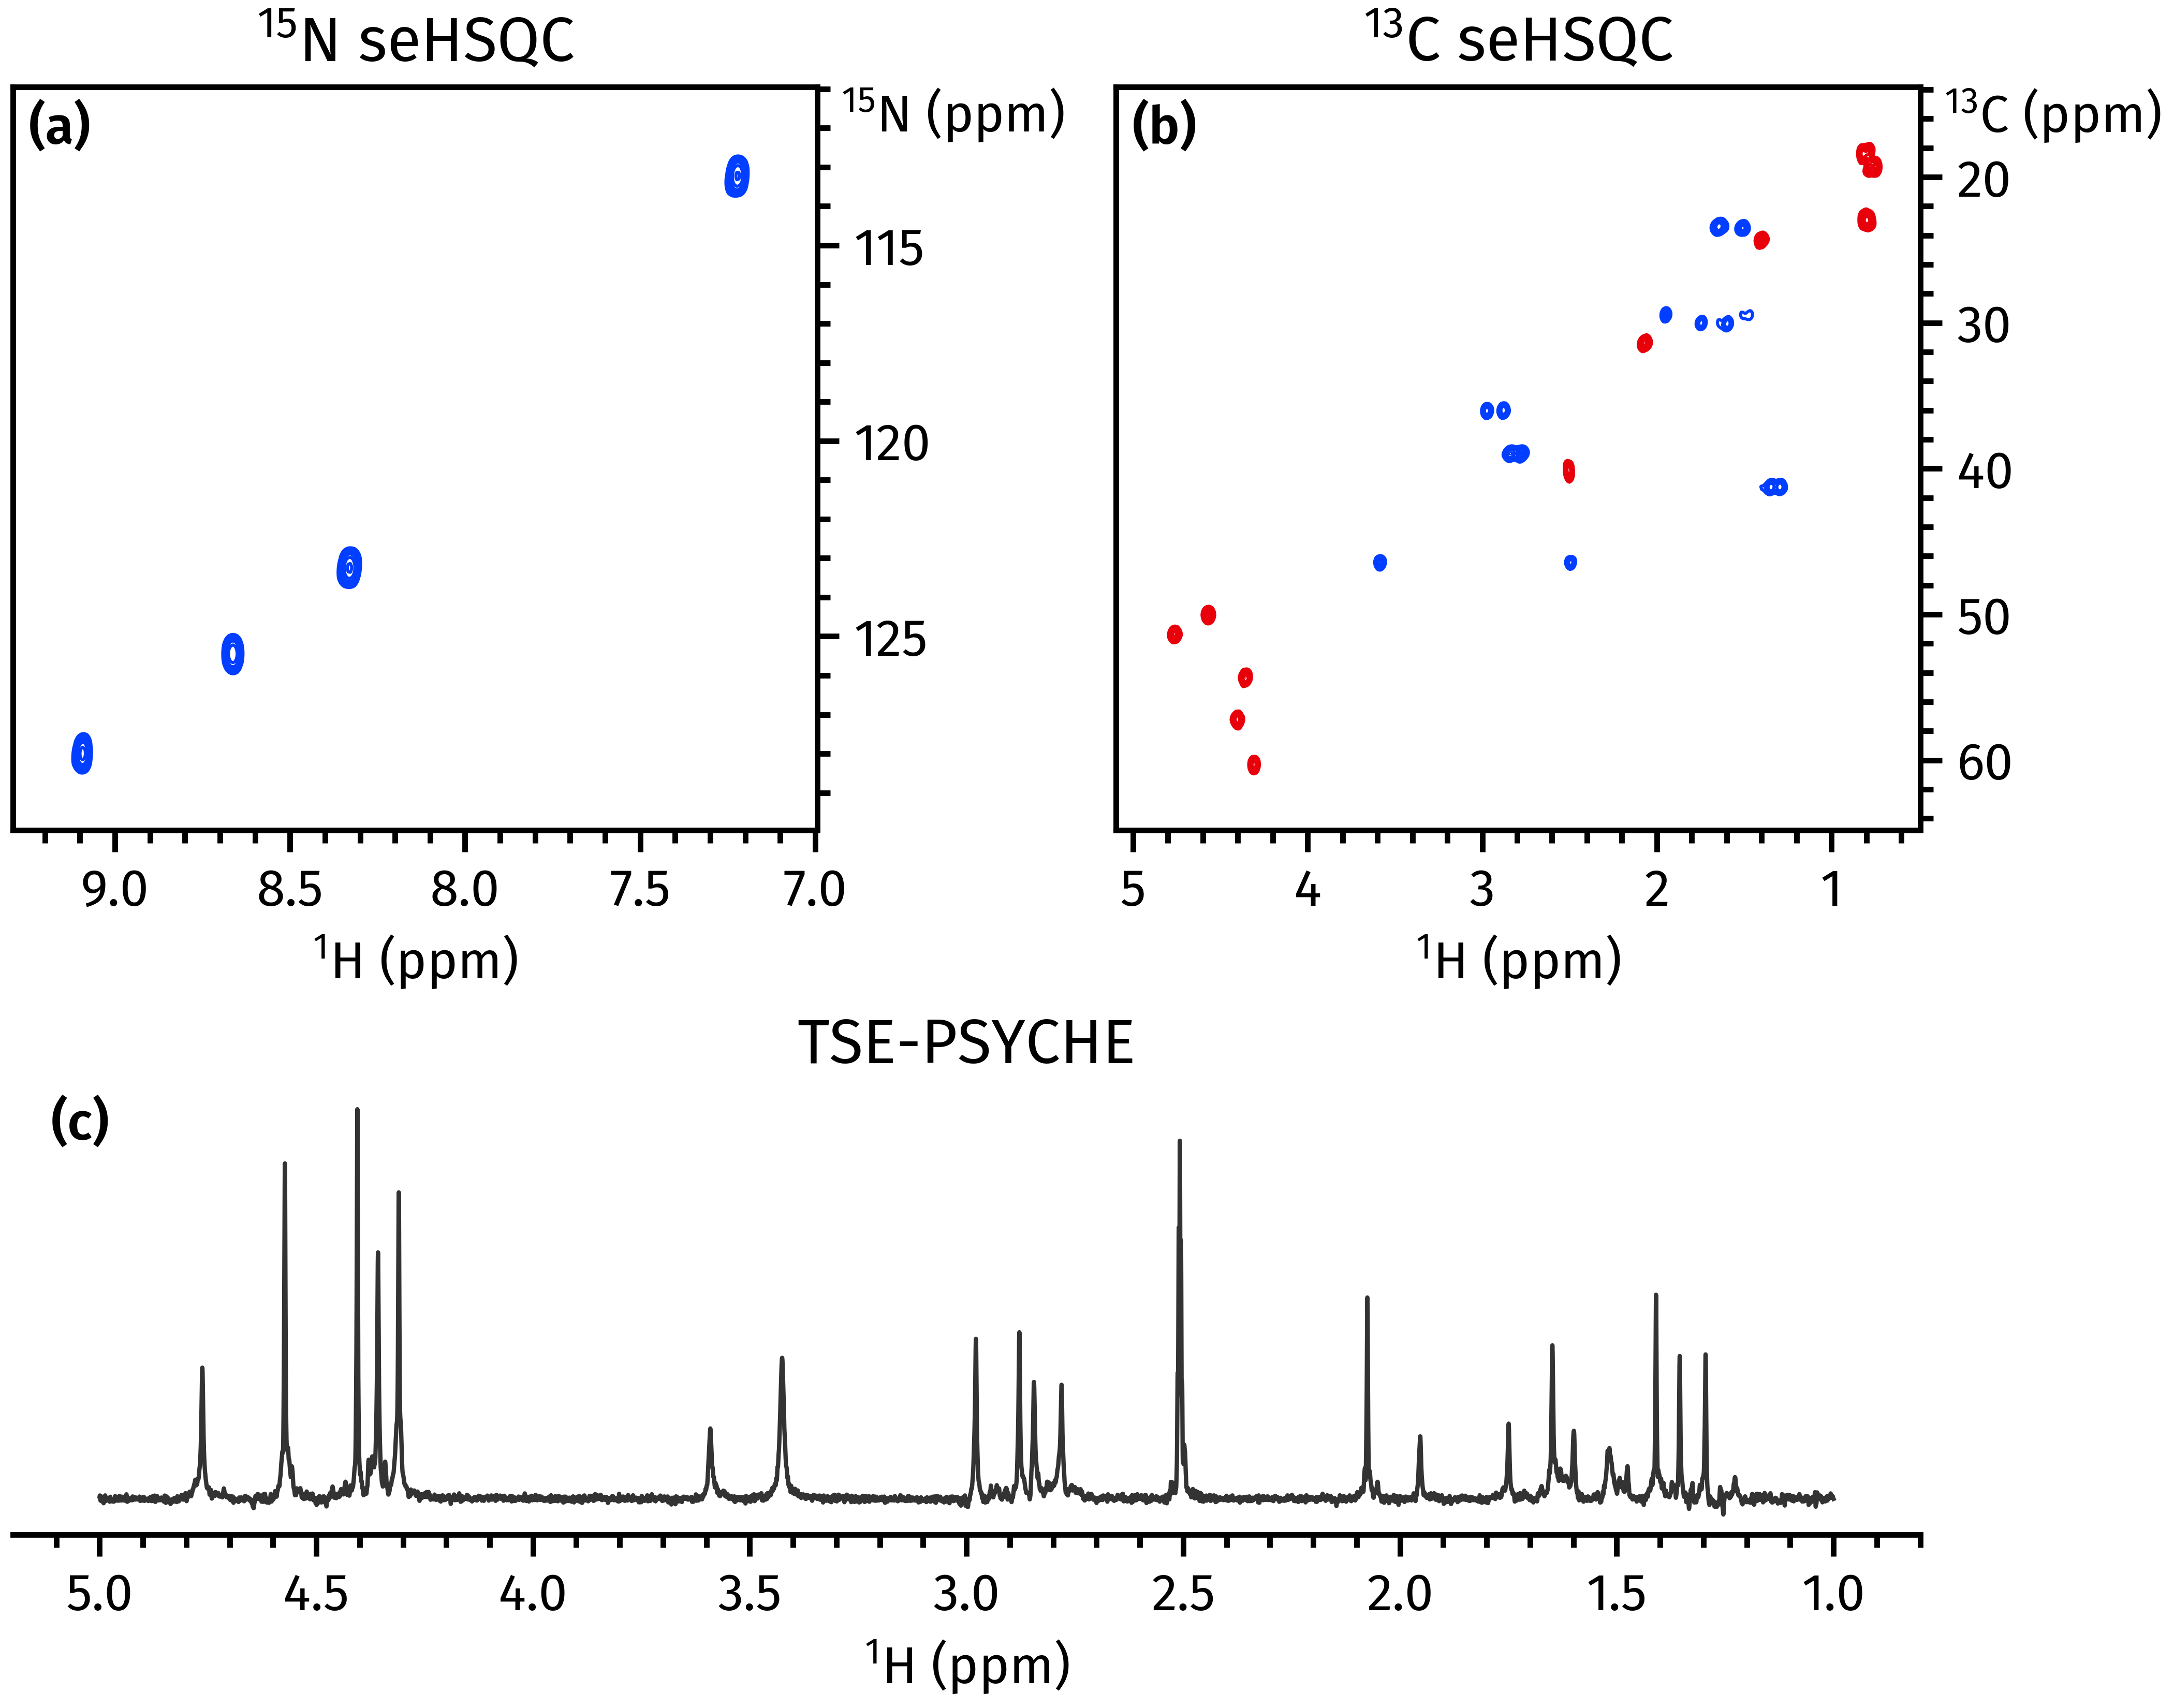
\includegraphics[width=0.7\textwidth]{psyche.png}
    {\phantomsubcaption\label{fig:psyche_n15_sehsqc}}
    {\phantomsubcaption\label{fig:psyche_c13_sehsqc}}
    {\phantomsubcaption\label{fig:psyche_psyche}}
    \caption{
        Spectra obtained from a NOAH-3 $\mathrm{S^{+}_{N}S^{+}P^T}$ supersequence.
        \textbf{(\subref{fig:psyche_n15_sehsqc})} \nitrogen{} sensitivity-enhanced HSQC\autocite{Yong2021JMR} (256 $t_1$ increments, 2 scans per increment).
        \textbf{(\subref{fig:psyche_c13_sehsqc})} \carbon{} sensitivity-enhanced HSQC\autocite{Hansen2021AC,Yong2021JMR} (256 $t_1$ increments, 2 scans per increment).
        \textbf{(\subref{fig:psyche_c13_sehsqc})} 1D TSE-PSYCHE pure shift spectrum\autocite{Foroozandeh2015CC} (saltire flip angle of \ang{10}, 32 chunks, 16 scans per chunk).
        \grami{}
    }
    \label{fig:psyche}
\end{figure}

A simple extension of this protocol to \textit{homonuclear} \proton{}--\proton{} modules enables experiments such as 2D J-resolved spectroscopy or pseudo-2D pure shift techniques to be incorporated into NOAH supersequences.
In both cases, the number of $t_1$ increments needed (16--32) is far smaller than the typical number required for a 2D experiment (128--256).
In particular, at present, we have implemented a family of PSYCHE experiments, namely the original pseudo-2D PSYCHE, the triple spin echo (TSE)-PSYCHE experiment which provides improved robustness towards strong coupling, and the PSYCHE 2DJ experiment which yields pure absorption-mode lineshapes.\autociteset{psyche}

In PSYCHE spectra, the flip angle of the chirp or saltire pulses used in the J-refocusing element provides the experimentalist with a choice: a larger flip angle provides greater sensitivity, but at the cost of increased artefacts.\autocite{Foroozandeh2018CEJ}
One advantage of acquiring PSYCHE spectra in NOAH-type supersequences is that, due to the increased number of transients, sensitivity is often not at a premium.
Thus, the user can choose a smaller flip angle (ca.\ \ang{10}) in order to maximise spectral purity instead, while not losing any actual spectrometer time.
An example of a NOAH-3 supersequence with the TSE-PSYCHE module is shown in \cref{fig:psyche}.

\subsection{splitx\_au processing}
\label{subsec:splitx_au}

NOAH data processing is done using the \texttt{splitx\_au} AU programme; this is responsible for creating \texttt{NBL} separate datasets containing the data for each module, and processing each dataset using module-specific AU programmes (e.g.\ \texttt{noah\_hsqc} for \carbon{} HSQC data).
Previously, the module-specific AU programmes had to be specified as the \texttt{USERP1}, \texttt{USERP2}, \ldots{} series of processing parameters.
Since the GENESIS approach allows module-specific information such as these to be embedded within the pulse programme itself, this means that (with a small modification to the \texttt{splitx\_au} AU programme) we can parse the pulse programme to obtain the requisite list of AU programmes.
The user therefore does not have to specify it explicitly, which makes setting up multiple different supersequences a much smoother process.
It is still possible to specify the \texttt{USERPx} parameters, and these will override the AU programmes parsed from the pulse programme, but in practice there is no real reason to do so.

\subsection{Non-uniform sampling implementation}

With the GENESIS pulse programmes we also introduce a new and more user-friendly implementation of non-uniform sampling (NUS).
NOAH experiments do not work ``out of the box'' with TopSpin's conventional NUS setup routine: some special adjustments have to be made by manually generating the list of increments to be sampled and adjusting the $t_1$ delays accordingly.
Previously, this was accomplished using a Python script which created a new pulse programme for each supersequence, e.g.\ \texttt{noah3\_BSC.nus}.\autocite{Claridge2019MRC}
We have modified this approach such that the \textit{same} pulse programme can be used for both uniform and non-uniform sampling, where NUS is controlled by an acquisition flag \texttt{-DNUS}.
Although a (different) Python script is still required for initialisation, this means that it is no longer necessary to keep two separate instances of the same pulse sequence in TopSpin, and reduces the difficulty of turning NUS on and off.


\section{Conclusion}

\todo{To be written.}

% Fakesection Bibliography
\printbibliography{}

% Fakesection SI preamble-like commands
\clearpage
\newcommand{\sectionbreak}{\clearpage}
\renewcommand*{\thefigure}{S\arabic{figure}}
\renewcommand*{\thesection}{S\arabic{section}}
\renewcommand*{\thetable}{S\arabic{table}}
\renewcommand*{\thepage}{S\arabic{page}}
\setcounter{page}{1}
\setcounter{figure}{0}
\setcounter{section}{0}
\setcounter{table}{0}
\onehalfspacing

\section{Number of combinations}
\label{sec:combinations}

In this section we count the total number of ``plausible'' NOAH combinations, available from the non-developer mode version of the GENESIS website, using the inclusion--exclusion principle.
As of version \todo{2.0.12} of the website, there are five categories of modules:
\begin{itemize}
    \item HMBC (\the\nmoda{} choices, including ``none'')
    \item \NH{} (\the\nmodb{} choices, including ``none'')
    \item \CH{} \#1 (\the\nmodc{} choices, including ``none'')
    \item \CH{} \#2 (\the\nmodd{} choices, including ``none'')
    \item \HH{} (\the\nmode{} choices, including ``none'')
\end{itemize}

To a first approximation, there are therefore
\(\the\nmoda{} \cdot \the\nmodb{} \cdot \the\nmodc{} \cdot \the\nmodd{} \cdot \the\nmode{} = \mathbf{\ee{\nmoda*\nmodb*\nmodc*\nmodd*\nmode}}\)
combinations.
Since we included the ``none'' options in this product, this figure includes ``lesser'' supersequences such as NOAH-4 and lower.
However, this does contain some invalid combinations, namely:
\begin{enumerate}
    \item All five ``none'' modules selected (\(\mathbf{1}\)).
    \item ``NOAH-1'' combinations with only one module: \(\ee{\nmoda-1} + \ee{\nmodb-1} + \ee{\nmodc-1} + \ee{\nmodd-1} + \ee{\nmode-1} = \mathbf{\ee{\nmoda+\nmodb+\nmodc+\nmodd+\nmode-5}}\).
        These are technically valid experiments (and the pulse programmes generated by the website \textit{will} function correctly), but they are no different from standard 2D experiments so the NOAH description does not truly apply to these.
    \item ``NOAH-6'' combinations where there is one experiment in each of the first four categories, and a ``double'' experiment (e.g.\ COSY + NOESY) in the last category.
        There are \(\ee{\nmoddoublehom}\) such modules, for a total of \(\ee{\nmoda-1} \cdot \ee{\nmodb-1} \cdot \ee{\nmodc-1} \cdot \ee{\nmodd-1} \cdot \ee{\nmoddoublehom} = \mathbf{\ee{(\nmoda-1)*(\nmodb-1)*(\nmodc-1)*(\nmodd-1)*\nmoddoublehom}}\) combinations.
        These are perfectly sound from a scientific perspective, but cannot be executed in current versions of TopSpin as the parameter \texttt{NBL} (number of modules) has a maximum value of 5.
    \item NOAH-2 or NOAH-3 combinations consisting of the HMBC module directly followed by a \HH{} homonuclear module: \(\mathbf{\ee{\nmode-1}}\).
        These can be run, but are likely to produce lower-quality homonuclear spectra as the HMBC module dephases bulk magnetisation.
    \item Duplicate, identical combinations where the same \CH{} module (e.g.\ HSQC) was selected either from the third or the fourth column.
        There are \(\ee{\nmoddup}\) such modules, so we must subtract \(\ee{\nmoda} \cdot \ee{\nmodb} \cdot \ee{\nmoddup} \cdot \ee{\nmode} = \mathbf{\ee{\nmoda*\nmodb*\nmoddup*\nmode}}\) combinations.
        \begin{itemize}
            \item Note, however, that some of these duplicate combinations were \textit{already} rejected in step (2) above. Thus, we need to add back \(\mathbf{\ee{\nmoddup}}\) ``NOAH-1'' combinations that we double-counted.
        \end{itemize}
\end{enumerate}

This yields a total number of
\(\mathbf{ %
    \ee{\nmoda*\nmodb*\nmodc*\nmodd*\nmode} %
    - 1 %
    - \ee{\nmoda+\nmodb+\nmodc+\nmodd+\nmode-5} %
    - \ee{(\nmoda-1)*(\nmodb-1)*(\nmodc-1)*(\nmodd-1)*\nmoddoublehom} %
    - \ee{\nmode-1} %
    - \ee{\nmoda*\nmodb*\nmoddup*\nmode} %
    + \ee{\nmoddup} %
    = \ee{(\nmoda*\nmodb*\nmodc*\nmodd*\nmode)-1-(\nmoda+\nmodb+\nmodc+\nmodd+\nmode-5)-((\nmoda-1)*(\nmodb-1)*(\nmodc-1)*(\nmodd-1)*\nmoddoublehom)-(\nmode-1)-(\nmoda*\nmodb*\nmoddup*\nmode)+(\nmoddup)} %
}\)
possible NOAH supersequences.
Note that, unlike the original paper\autocite{Kupce2017ACIE}, this does not take into account options that are set using acquisition flags, such as multiplicity editing in HSQC-type experiments and inversion of ``indirect'' responses in HSQC-COSY and HSQC-TOCSY spectra.
This also does not include modules that are only available via the ``developer mode'' interface.

\end{document}
